\documentclass[conference]{IEEEtran}

\usepackage{cite}
\usepackage{listings}
\usepackage{amsmath}
\lstset{showstringspaces=false, basicstyle=\footnotesize, numbers=left, numbersep=1pt }
\usepackage[tableposition=top]{caption}
\ifCLASSINFOpdf
\usepackage[pdftex]{graphicx}
\usepackage[pdftex]{color}
\usepackage{subcaption}
\else
\fi
\usepackage{url}
\usepackage{upquote}


\hyphenation{op-tical net-works semi-conduc-tor}


\begin{document}\title{SpyREST in Action: Demo of an Automated RESTful API Documentation Tool}

\author{\IEEEauthorblockN{S M Sohan, Craig Anslow, and Frank Maurer}
\IEEEauthorblockA{Department of Computer Science\\
University of Calgary\\
Calgary, Alberta T2N 1N4\\
Email: \{smsohan, craig.anslow, frank.maurer\}@ucalgary.ca  }
}
\maketitle


\begin{abstract}
RESTful APIs are often manually documented. As a result, the process is both expensive and error-prone to maintain the documentation of RESTful APIs over time. In this demonstration paper, we present SpyREST as an automated software as a service tool that can be used to document RESTful APIs. SpyREST leverages a HTTP Proxy server to intercept real API calls to automatically collect and generate RESTful API documentation by synthesizing HTTP traffic involved in API calls. SpyREST provides an automated yet customizable documentation solutions for RESTful APIs. The generated documentation includes both the API references as well as executable API examples and collaboration features. RESTful API developers can use SpyREST to auto generate and publish documentation for their APIs instead of using a manual approach.

\end{abstract}

\IEEEpeerreviewmaketitle

\section{Overview}

\subsection{How SpyREST Works?} % (fold)
\label{sub:how_it_works}

SpyREST is a web-based software as a service tool that can be accessed at http://SpyREST.com. To auto-generate documentation for RESTful APIs, SpyREST relies on HTTP traffic information captured while example API calls are made using a HTTP proxy. The high level process can be described as a 3 step process: API developers make example API calls using a HTTP proxy server, the HTTP proxy server captures the HTTP headers, request and response data, the collected data is synthesized and presented on a web application.

The proxy server used in SpyREST is a ``value-added'' one specialized for RESTful API documentation. A typical HTTP proxy server can intercept and record the HTTP traffic for example API calls but further processing is required to generate a usable RESTful API documentation out of it. For example, API reference documentations need to be version aware so that the documentation can clearly refer to the relevant API versions. To provide human readable description to the example API calls, relevant information needs to be captured in addition to the raw HTTP traffic. Post processing is required to generate the structure of request and response payloads by parsing and consolidating raw HTTP data from multiple example API calls since the optional fields may not be obvious when looked at individual example calls.

To generate usable documentation, SpyREST automatically parses the captured HTTP request and response data and presents summary tables showing the structure for HTTP query parameters, headers, request and response data. For each field, SpyREST displays the name of the field, example values and automatically inferred data type information such as integer, date time, etc. To reduce verbosity from large API responses, SpyREST automatically strips large responses to only show representative samples from repeated values in arrays. SpyREST does not capture and strip off any authorization header used in the example API calls to prevent confidential information from being part of the documentation.


\begin{figure}[tbh]
  \centering
  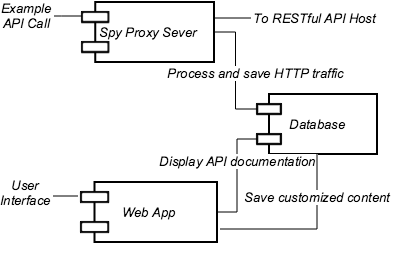
\includegraphics[width=\linewidth]{spyrest_components.png}
  \caption{SpyREST Component Diagram}
  \label{fig:components}
\end{figure}

By using a HTTP proxy server, SpyREST enables the documentation of different RESTful APIs independent of the implementation technology behind the APIs. Since SpyREST is offered as a software as a service tool, it can be used as a reusable platform for generating and publishing documentation of many different RESTful APIs. When isolation is desired, SpyREST can also be used as a self-hosted tool. SpyREST is released as an open-source product and for self-hosted solutions it can be customized to fit unique requirements.

The web interface of SpyREST provides a hierarchical navigation for RESTful API documentation as follows: each API host has one or more API versions, each API version has one or more resources, each API resource has one or more API actions, each API action may have a structure of HTTP query parameters, headers, request and response payloads as well as many API examples, each API example may have HTTP query parameters, headers, request and response payloads. The web interface also provides a wiki-like editor to allow API developers to override auto generated API documentation using Markdown syntax. On each page, the web interface includes collaboration features so that API developers can discuss questions and collect feedbacks about specific API documentation pages. For each API example, SpyREST generates a cURL command that can be run to execute the API examples without writing any code.


\subsection{Implementation} % (fold)
\label{sub:implementation}

SpyREST is composed of three main components as shown in Fig. \ref{fig:components}. The ``Spy'' component is the ``value-added'' HTTP proxy server. This component is written using NodeJS. The Spy has internal logic to decode HTTP request URL and headers and auto-detect API versions for the commonly used version identifier patterns. The Spy also parses the URL to auto detect the API resources, API actions and query parameters for the example API calls. Even though the auto detected API version, resource and actions cover the commonly observed patterns, API developers can override the auto-detections of any of these fields by using custom Spy specific HTTP headers when making the example API calls. The HTTP headers x-spy-rest-version, x-spy-rest-resource, and x-spy-rest-action can be used to override auto-detection of these respective fields. Additionally, API developers can use x-spy-rest-desc header to attach human readable descriptions for each API example so that the web interface can tag the examples against meaningful descriptions.


The Web App component is implemented using Ruby on Rails. To allow RESTful API developers to edit auto generated documentation, it uses the popular GitHub Flavored Markdown. To facilitate collaboration across all the API documentation pages, the Web App uses Disqus, a popular third-party collaboration service.

The Spy writes the captured and synthesized API example data into a MongoDB database. The Web App reads and saves custom edits on the same database. The technology choice behind for our implementation of SpyREST components is based on our past experience of using these tools but the concepts behind SpyREST is not dependent on the aforementioned technology choice. As a proof of concept, SpyREST only analyzes JSON based API request and response payloads because of its popularity among modern day RESTful APIs.

All three SpyREST components are released as docker containers. Docker is a popular lightweight visualization solution that can either be hosted in-house or using many of the popular cloud hosting providers. The public instance of SpyREST (http://SpyREST.com) has the three components in three separate docker containers running on a single linux server with 512MB memory, 1 core processor, and 20GB disk space.

\section{Use Cases}
In this section, we describe two different use cases from the perspective of initially generating a RESTful API documentation for the first time and maintaining the documentation over time as the API evolves.

\begin{figure*}[tbh]
  \centering
  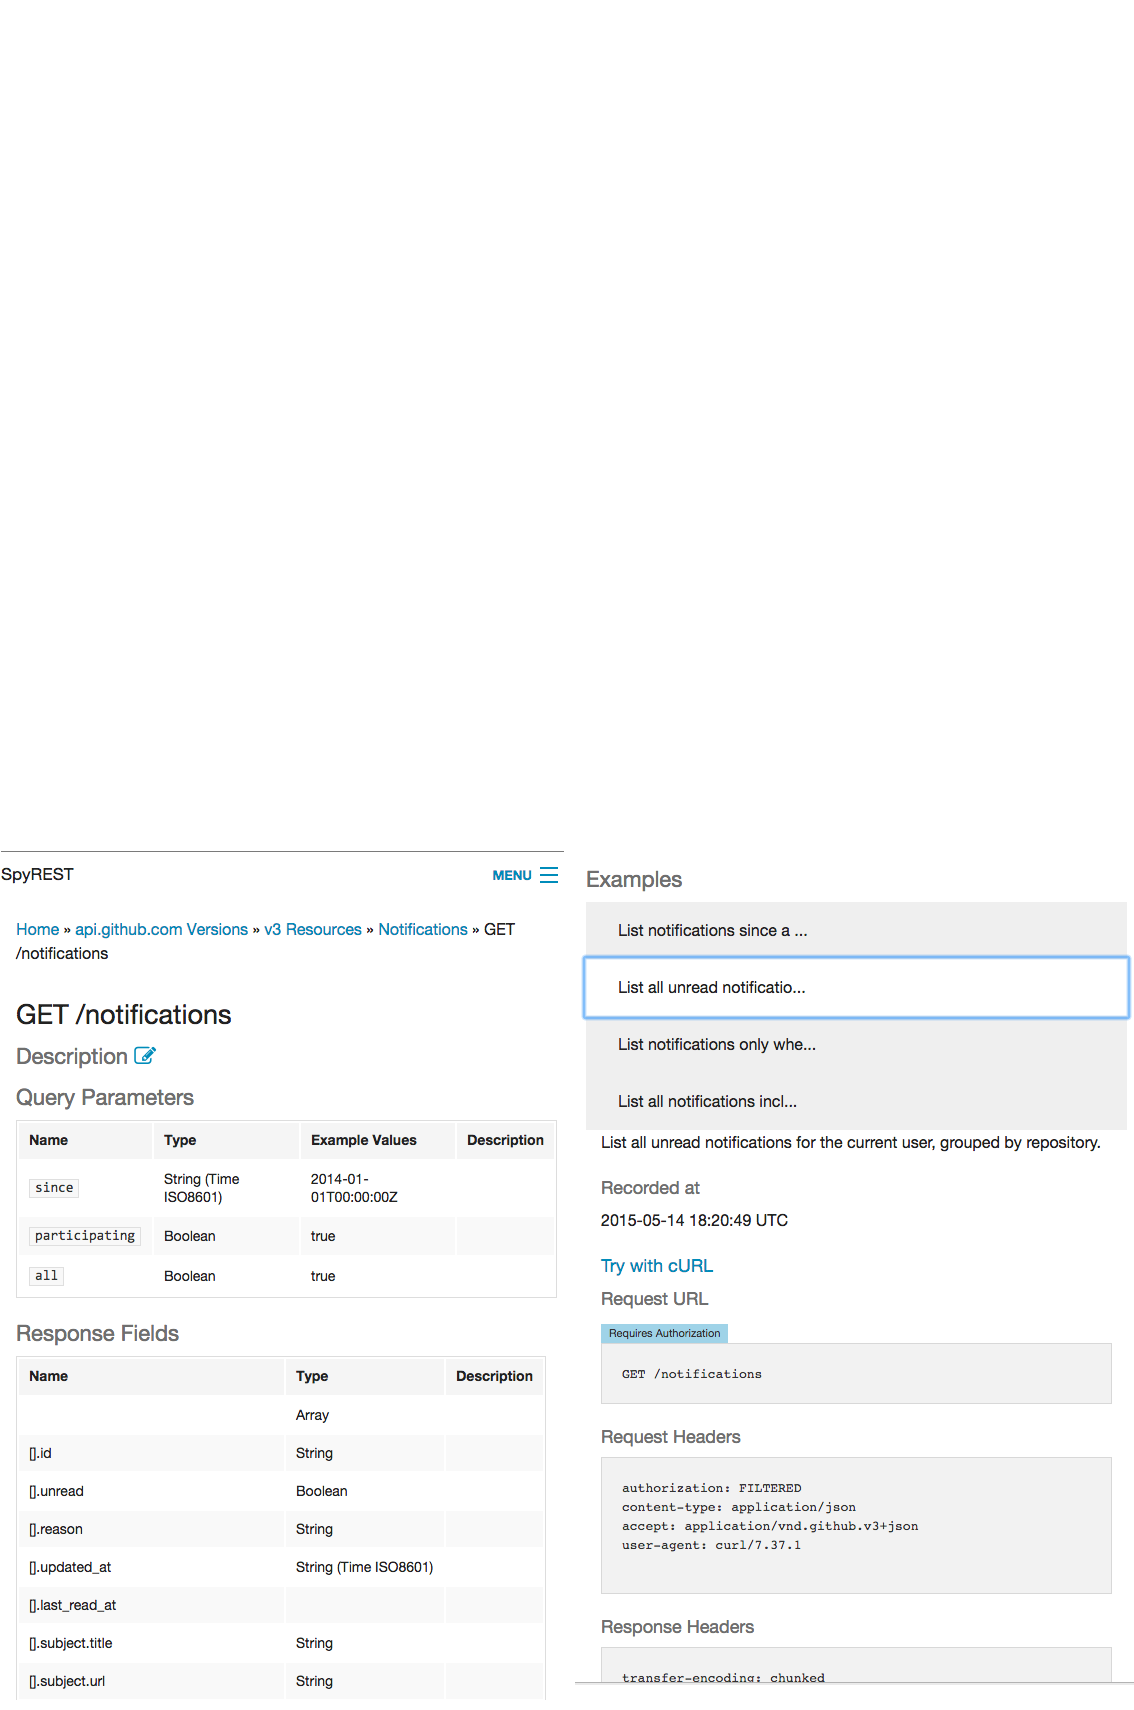
\includegraphics[width=0.8 \linewidth]{notifications.png}
  \caption{SpyREST Partial Screen shot}
  \label{fig:screenshot}
\end{figure*}

\subsection{Initial API Documentation} % (fold)
When releasing a RESTful API, API developers need to publish the API documentation so that other developers can use the APIs. For demonstration, let's consider generating a documentation for the ``GET /notifications (List your notifications)'' API that is exposed by GitHub\footnote{\url{https://developer.github.com/v3/activity/notifications/#list-your-notifications}}. Using this API a developer can paginate through the list of all public repositories within GitHub. This API action takes an optional parameter ``since'' that can be used to specify a time filter.

To manually generate a documentation for this API, a developer needs to follow these steps: 1) make example authenticated API calls to $GET /notifications$, 2) record the HTTP headers with request and response data, 3) remove duplicate information, 4) remove authentication information, 5) format and stylize the reduced information, 6) add custom content, 7) organize multiple formatted documents together on a web site with navigation, and 8) publish the documentation website. This step needs to be repeated for each of the API endpoints. Since this is a manual process, there is also a room for human errors in the aforementioned steps. SpyREST aims to automate all but steps 1 and 6 of this process.

To use SpyREST for auto-generating the documentation of this API, an API developer only needs to make the example API calls via the Spy proxy server with custom HTTP headers for human readable descriptions for the API examples. If desired, custom edits to the auto generated documentation may be made by using the Markdown editor. Fig \ref{fig:screenshot} shows a partial screen shot of SpyREST generated documentation for this API given 4 example API calls. SpyREST fully automates the steps 2-5, and 7-8 and so that API developers only need to focus on finding good example API calls and describing the complex rules about APIs that are not otherwise derivable from looking at the request and response data alone. In addition to automating the RESTful API documentation process, SpyREST also displays a cURL command for each recorded API example so that developers can try the API examples without having to write any code. In page collaboration allows the users to discuss API related questions and find past conversation all in one place. In this specific example, we see the official documentation of $GET /notifications$ provided by GitHub was outdated and missing several fields (e.g. $subscription\_url$, $repository.releases\_url$, $repository.labels\_url$, $repository.notifications\_url$ and 28 more) that are automatically documented by SpyREST.

\subsection{Maintaining API Documentation for evolving APIs} % (fold)
Maintenance of RESTful API documentation is another use case of interest since the documentation for RESTful APIs need to evolve with the APIs to reflect the updated information. The 8 steps mentioned previously need to be repeated every time any of the API objects changes when a manual process is followed. Since APIs continue to evolve throughout its lifetime, manually maintaining their documentation incurs further cost or causes the outdated documentation.

SpyREST automatically updates the recorded information for each example API call, so rerunning the API examples automatically updates the auto-generated documentation. To uniquely identify each example API call, the Spy computes a SHA1 based digital signature of example API call based on its API version, resource, URL and custom description. To replay the example API calls, API developers can use automated scripts so that once an API example is scripted, it can be run repeatedly. Moreover, the automated scripts can be written as functional tests where the generation of API documentation becomes a side-benefit of running the tests. Running the automated scripts to exercise the API examples frequently can prevent out of date API documentations as shown on the previous use case.

\begin{lstlisting}[language=ruby, breaklines=true, caption={}, label=list:ex, float,floatplacement=H, caption=Example API call using SpyREST, label={lst:notifications}]
class Github

  include HTTParty

  base_uri 'https://api.github.com'
  headers('Accept' => 'application/vnd.github.v3+json',
    'User-Agent' => 'curl/7.37.1',
    'content-type' => 'application/json',
    'Authorization' => "token GITHUB_API_TOKEN'"
  )

  host, port = 'spyrest.com', 9081
  http_proxy host, port

end

describe 'Notifications' do

  it 'List all notifications for the current user, where they are participating, since a time' do

    response = Github.get '/notifications?all=true&participating=true&since=2014-01-01T00:00:00Z'
    assert_equal 200, response.code
  end

end\end{lstlisting}

Listing \ref{lst:notifications} shows an example script written using Ruby based test framework Minitest. In this example script, the class $Github$ is setup with connection information so that it uses the Spy proxy server to make example API calls. Then, on line 21 we make an example API call which automatically generates a documentation for the $GET /notifications$ API action. The results of the API call can be used to test against expected results. Using this 25 line script a developer may generate the documentation for this API and auto-update the documentation by rerunning the script anytime the API changes while still getting test coverage.

\section{Discussion}
With SpyREST we have aimed to provide an automated solution to the RESTful API documentation problem since a manual approach to generate and maintain RESTful API documentation is both expensive and error-prone.


\section{Related Work}
Page 5

\section{Conclusion}
Page 5

\end{document}


